\documentclass[12pt,onecolumn,a4paper]{article}
\usepackage{epsfig,graphicx,amsthm,amsmath}
\usepackage{color,xcolor}
\usepackage{fancyvrb}
\usepackage{enumerate}
\usepackage{caption}
\usepackage{subcaption}
\usepackage{pgfplots}
\usepackage{hyperref}
\usepackage{lscape}
\usepackage{booktabs}
\usepackage{xepersian}
\settextfont[Scale=1.0]{Far.Roya}
\setlatintextfont[Scale=1]{Times New Roman Cyr}

\begin{document}

\begin{titlepage}
\title{گزارش پروژه‌ی رایانش چند هسته‌ای \\ \lr{Edge Detection Filter}} 
\author{نوید اسلامی - 98100323 \\ سروش جهان‌زاد - 98100389}
\date{\today}
\maketitle
\end{titlepage}

موضوع پروژه‌ای که در نظر گرفته‌ایم، \lr{Edge Detection} به کمک فیلتر \lr{Sobel} است. درواقع با استفاده از دو \lr{Convolution}ای که مشتق‌های در راستای $x$ و $y$ را محاسبه می‌کند، یک تخمین از نرم مشتق کلی به دست می‌آوردیم و بر حسب آن یک تصویر خروجی ایجاد می‌کنیم که نقاط سفید به معنی وجود گوشه و نرم بزرگ‌تر مشتق است و نقاط سیاه به معنی یکنواختی عکس است. حال به توصیف روند و تکنیک‌های مورد استفاده در پیاده‌سازی خود می‌پردازیم.

\section{پیاده‌سازی و بهینه‌سازی‌های مورد استفاده}
در درجه‌ی اول، تصمیم گرفتیم که عمل تغییر \lr{Brightness} را به صورت یک کرنل جدا از خود عمل فیلتر کردن تعریف کنیم. بعد از تغییر \lr{Brightness} اما، تصویر ورودی را که فرض کرده‌ایم می‌تواند رنگی نیز باشد، به سیاه و سفید تبدیل می‌کنیم. (با میانگین‌گیری مقادیر کانال‌ها) همچنین تصمیم گرفتیم که عمل \lr{Thresholding} را با استفاده دو مقدار \lr{Threshold} $t_1$ و $t_2$ انجام دهیم، به این صورت که پیکسل‌های خروجی‌ای که مقداری کمتر از $t_1$ داشتند را صفر کنیم و پیکسل‌های با مقدار بیشتر از $t_2$ را کاملاً روشن کنیم. همچنین، برنامه‌ی مذکور را طوری پیاده‌سازی کرده‌ایم که بتواند هر اندازه تصویری را به درستی هندل کند، حتی تصاویر خیلی بزرگ مثل تصاویر \lr{8K}. در پیاده‌سازی این پروژه، ابتدا کد اصلی و رابط کاربری \lr{CLI} را پیاده‌سازی کردیم و سپس به آن \lr{GUI} اضافه کردیم.

\subsection{پیاده‌سازی \lr{CLI}}
ابتدا به کمک کتاب‌خانه‌ی \lr{OpenCV}، تصویر مربوطه را از فایل می‌خوانیم. سپس، مقادیر ثابت الگوریتم را مثل تغییر روشنایی تصویر و نیز \lr{Threshold}ها را تعریف می‌کنیم. در ادامه، داده‌هایی که نیاز داریم را در حافظه‌ی \lr{GPU} در اختیار می‌گیریم. تصویر خوانده شده را با یک سطر صفر از بالا و $channel \; count$ سطر صفر از پایین \lr{Pad} می‌کنیم تا بتوانیم الگوریتمی که در \lr{GPU} اجرا می‌کنیم را راحت‌تر پیاده‌سازی کنیم. توجه کنید اما که قبل از این صفر کردن‌ها، صرفاً تصویر اصلی ورودی را در مکان مناسب و مذکور کپی می‌کنیم و آن را با استفاده از کرنل مخصوص \lr{change{\_}brightness}، مطابق با ورودی ثابت آن روشن‌تر یا تاریک‌تر می‌کنیم.

این کرنل، صرفاً تک تک پیکسل‌ها را که به صورت یک سطر بزرگ در آرایه‌ی خوانده شده ذخیره شده‌اند را تغییر می‌دهد. با استفاده از بلوک‌ها و گرید‌های مختلف، ریسه‌ها را مسئول تغییر اجزای مختلف تصویر مذکور می‌کنیم. هر ریسه نیز برای عملکرد بهتر، از تکنیک \lr{Loop Unrolling} استفاده می‌کند و درواقع 4 مقدار کانال متوالی را هندل می‌کند. همچنین، خود این هندل کردن نیز را طوری نوشته‌ایم که به صورت \lr{Branchless} اجرا شود و در نتیجه، بتوانیم سرعت و بهره‌وری بالاتری را در اجرای برنامه‌های خود داشته باشیم. با تکرار همین فرآیند و هندل کردن شیفت‌ها مختلف از مقادیر کانال‌ها، تغییر میزان روشنایی هر کانال را به خوبی انجام می‌دهیم و از پرش اضافه‌ای استفاده نمی‌کنیم. توجه کنید که از آن‌حایی که این مقادیر صرفاً بایت هستند، هندل کردن چهار مقدار معادل هندل کردن یک کلمه است. در نتیجه، \lr{Loop Unrolling} به این شکل مشکلی برای \lr{Cache Locality} ایجاد نمی‌کند و صرفاً تعداد دستورات اضافه‌ای که باید اجرا شود را کمینه می‌کند. با اتمام این فرآیند پس، تصویر خود را روشن‌تر و یا تاریک‌تر می‌کنیم و در همان آرایه‌ی ورودی ذخیره می‌کنیم تا بتوانیم بعداً از آن به راحتی استفاده کنیم.

بعد از تغییر روشنایی تصویر، پردازنده‌ی اصلی را با \lr{GPU} همگام می‌کنیم تا بتوانیم به صورت امن اعمال بعدی را انجام دهیم. در این مرحله، سطر‌های صفری که برای \lr{Padding} نیاز داشتیم را به کمک \lr{cudaMemset} صفر می‌کنیم و آرایه‌ای که باید تصویر خروجی را در خودش ذخیره کند را در حافظه‌ی \lr{GPU} می‌گیریم. در این لحظه نیز، اندازه‌ی بلوک‌ها و گرید را تنظیم می‌کنیم تا بتوانیم فیلتر را اعمال کنیم. در ادامه، با استفاده از این مقادیر، کرنل \lr{tiled{\_}sobel} را فراخوانی می‌کنیم تا فیلتر را اعمال کند.

کرنل مذکور، برای این که بتواند خروجی را به خوبی تولید کند، از ایده‌ی \lr{Tiling} استفاده می‌کند. به عبارتی، هر بلوک از ریسه‌های یک بخش به طول 128 و عرض 8 پیکسلی از ورودی را هندل می‌کند و به آن فیلتر را اعمال می‌کند. همچنین، کد را طوری زده‌ایم که بلوک‌های داخل یک گرید بتوانند با شیفت دادن خود به هندل کردن بخش‌های مشابه بعدی از تصویر بپردازند، بدون این که \lr{Cache Locality} را خیلی ه هم بریزند. برای این که بتوانیم از \lr{Data Sharing} حاصل از این ایده استفاده کنیم، از حافظه‌ی مشترک \lr{GPU} نیز استفاده می‌کنیم. به این شکل عمل می‌کنیم که پیکسل‌های مربوط به هر بخش از تصویر که برای یک بلوک است، و نیز پیکسل‌های مجاور آن بخش را ابتدا به سیاه و سفید تبدیل می‌کنیم (سه بایت ورودی به یک بایت سیاه سفید در $smem$ تبدیل می‌شود) و مقادیر تبدیل شده‌ی حاصل را در یک ساختار کاملاً مشابه در حافظه‌ی مشترک $smem$ ذخیره می‌کنیم.

در همین راستا، ابتدا قسمت میانی بخش مربوط به یک بلوک را هندل می‌کنیم و به صورت \lr{Branchless} بررسی می‌کنیم که آیا پیکسلی که باید لود شود واقعا داخل تصویر هست یا نه. در صورتی که تبود، چون بلوک ما حافظه‌ی مشترکی برای خود دارد، می‌تواند به راحتی و بدون نگرانی صرفاً در آن‌ها صفر ذخیره کند. همچنین توجه کنید که حافظه‌ی مشترک ما \lr{Row Major} اختصاص داده شده است، اما اندیس هر ریسه اول $x$هایش عوض می‌شود و سپس $y$هایش. در نتیجه، برای این که \lr{Bank Conflict} نداشته باشیم، از $smem$ طوری استفاده می‌کنیم که $y$ مربوط به شماره‌ی سطر باشد و $x$ مربوط به شماره‌ی هر عنصر در هر سطر باشد. در نتیجه، به این شکل دسترسی‌های به حافظه در این حالت متوالی خواهند شد و مشکلی سر \lr{Bank Conflict} نخواهیم داشت. در ادامه، باز سعی کرده‌ایم که بدون پرش عناصر مرزی بخش مربوط به بلوک را در $smem$ بیاوریم. اما در این حالت نیاز بود که یک شرطی داشته باشیم، که سعی شده است صرفاً از آن یک شرط استفاده شود. در نتیجه، با استفاده از روابط ریاضی‌ای که در کد مشهود است، ابتدا دو ستون چپ و راست و بخش میانی سطرهای بالا و پایین (به جز دو پیکسل اول و آخر آن‌ها) را می‌آوریم و در $smem$ ذخیره می‌کنیم. در آخر نیز به روشی کاملاً مشابه، 4 پیکسلی که جا مانده بود را لود می‌کنیم. این کار را به این دلیل انجام داده‌ایم که پیاده‌سازی ساده‌تری داشته باشد.

توجه کنید که وجود \lr{Padding}هایی که قبل‌تر ایجاد کردیم در این مرحله خیلی مهم می‌شود، چون دیگر لازم نیست شرطی را برای وجود پیکسل‌های بالا و پایین چک بکنیم و فقط کافی است که شروط بیرون زدن از چپ و راست را بررسی کنیم. این موضوع نیز \lr{Divergence} خیلی کمی را ایجاد می‌کند، چون صرفاً در تعداد خیلی کمی از \lr{Warp}ها ریسه‌ای مشغول اجرا کد داخل شرط می‌شود. در آخر تمام این محاسبات نیز، برای این که محاسبات فاز بعد که فیلتر را اعمال می‌کنیم به درستی پیش برود، ریسه‌های بلو را با دستور \lr{\_\_{synchthreads}} همگام می‌کنیم. این باعث می‌شود که تمام پیکسل‌های مربوط به بخش مذکور در $smem$ به طور کامل لود شوند و در محاسبات آینده خدشه‌این ایجاد نشود.

در ادامه، چون هر پیکسل داخل بخش بخش مربوطه که مرزی نیست تمام همسایگی‌اش را دارد، می‌تواند به راحتی مشتق‌های $x$ و $y$اش را محاسبه کند. این کار را اما باید با دقت انجام داد و هر دو مشتق را همزمان با هم و از پیکسل بالا-چپ تا پایین-راست حساب کنیم. این به این دلیل است که به این شکل، خواندن‌های از $smem$ متوالی می‌شوند و \lr{Bank Conflict} خیلی کمی را خواهیم داشت. پس به این شکل، هر کدام از مشتق‌ها محاسبه می‌شود. در آخر نیز، با استفاده روش‌های \lr{Branchless}، بررسی می‌کنیم که هر مؤلفه از مشتق منفی هست یا نه و اگر منفی بود، با استفاده از روش‌های بیتی و \lr{Twos Complement} آن‌ها را منفی می‌کنیم. (رفتار مذکور را می‌توانید در کد مشاهده کنید) در آخر نیز این دو اندازه‌ی به دست آمده را با هم جمع می‌کنیم و در صورتی که پیکسل مربوطه در خروجی وجود داشت، با تکنیک‌های \lr{Branchless}، آن را در بازه‌ی $[0,255]$ می‌آوریم. این حاصل جدید را نیز با \lr{Threshold}ها مقایسه می‌کنیم و باز به صورت \lr{Branchless}، خروجی را روشن کامل و یا خاموش کامل می‌کنیم و یا حتی تغییری در آن ایجاد نمی‌کنیم. تمام این \lr{Branchless} بودن‌ها میزان \lr{Divergence} را خیلی کم می‌کند. در نهایت هم برای این که ریسه‌هایی که کارشان تمام شده است داده‌های $smem$ را خراب نکنند، باز دستور \lr{\_\_{synchthreads}} را اجرا می‌کنیم.

پس به این شکل، با استفاده از این بهبودها، بلوک‌های مختلف به هندل کردن بخش‌های مختلف از تصویر و خروجی آن می‌پردازند و حاصل را تولید می‌کنند. پس فقط کافی است که حاصل تولید شده را به همراه تصویر \lr{Brightness Changed} در \lr{CPU} بیاوریم و در فایل‌های مناسب ذخیره کنیم.

\subsection{پیاده‌سازی \lr{GUI}}
برای پیاده‌سازی رابط کاربری این پروژه، تصمیم گرفتیم که با استفاده از زبان برنامه‌نویسی پایتون و به کمک کتاب‌خانه‌ی \lr{Flask}، یک \lr{Web Server} ساده ایجاد کنیم که نقش رابط کاربری را بازی کند. این سرور هر بار با ورودی گرفتن مسیر فایل ورودی و مسیر‌های فایل‌های خروجی و نیز مقادیر ثابت مربوط به الگوریتم‌ها، می‌تواند هم برنامه‌ی \lr{CPU} و هم \lr{GPU} را اجرا کند و خروجی را در یک صفحه به نمایش بگذارد. همچنین، در صورت بروز هرگونه خطایی نظیر نبود \lr{CUDA} و یا ورودی غلط، پیام خطای مناسب را به ما نمایش خواهد داد.

تمام اعمال مذکور با استفاده از قابلیت‌های \lr{Flask} و نیز توابع و کتاب‌خانه‌های پایتون (نظیر \lr{OS}) پیاده‌سازی شده‌اند. خود شکل و شمایل صفحات اما با استفاده از فایل‌های \lr{HTML} ایجاد شده‌اند، که از آن‌جایی که پیاده‌سازی آن‌ها مرتبط با موضوع پروژه نیست، از توصیف آن‌ها صرف نظر می‌کنیم. با منطقی مشابه نیز، از توصیف عمیق‌تز منطق کد پایتون سرور نیز صرف نظر می‌کنیم.

\section{نمونه‌های اجرای برنامه}
نمونه‌هایی از اجرای این برنامه را می‌توانید در شکل‌های~\ref{Figure:01_1000x1500} تا \ref{Figure:Output_01_1920x1200} مشاهده کنید. همانطور که مشاهده می‌شود، با \lr{offset}های مختلف در تغییر روشنایی خروجی حاصل تغییر می‌کند. همچنین، پیاده‌سازی ما برای هر اندازه‌ای از تصویر کار می‌کند، حتی تصاویر \lr{8K}. (این شکل‌ها را برای کم کردن حجم فایل گزارش نیاورده‌ایم) توجه کنید که در تمام این خروجی‌ها \lr{Thresholding} با $t_1=20$ و $t_2=240$ انجام شده است.

همچنین می‌توانید اثر بودن و یا نبودن \lr{Thresholding} را در شکل~\ref{Figure:Threshold_Test} مشاهده کنید.

\begin{figure}
     \centering
     \begin{subfigure}[b]{0.3\textwidth}
         \centering
         \includegraphics[width=\textwidth]{Images/Brightness_Change_-50_01_1000x1500.png}
         \caption{$\text{\lr{offset}}=-50$.}
         \label{Figure:01_1000x1500_-50}
     \end{subfigure}
     \hfill
     \begin{subfigure}[b]{0.3\textwidth}
         \centering
         \includegraphics[width=\textwidth]{Images/Original_01_1000x1500.jpeg}
         \caption{تصویر اصلی.}
         \label{Figure:01_1000x1500_0}
     \end{subfigure}
     \hfill
     \begin{subfigure}[b]{0.3\textwidth}
         \centering
         \includegraphics[width=\textwidth]{Images/Brightness_Change_50_01_1000x1500.png}
         \caption{$\text{\lr{offset}}=50$.}
         \label{Figure:01_1000x1500_50}
     \end{subfigure}
\caption{تصویر $1000 \times 1500$ با تغییرات روشنایی آن.}
\label{Figure:01_1000x1500}
\end{figure}

\begin{figure}
     \centering
     \begin{subfigure}[b]{0.3\textwidth}
         \centering
         \includegraphics[width=\textwidth]{Images/Output_-50_01_1000x1500.png}
         \caption{$\text{\lr{offset}}=-50$.}
         \label{Figure:Output_01_1000x1500_-50}
     \end{subfigure}
     \hfill
     \begin{subfigure}[b]{0.3\textwidth}
         \centering
         \includegraphics[width=\textwidth]{Images/Output_0_01_1000x1500.png}
         \caption{حاصل اصلی.}
         \label{Figure:Output_01_1000x1500_0}
     \end{subfigure}
     \hfill
     \begin{subfigure}[b]{0.3\textwidth}
         \centering
         \includegraphics[width=\textwidth]{Images/Output_50_01_1000x1500.png}
         \caption{$\text{\lr{offset}}=50$.}
         \label{Figure:Output_01_1000x1500_50}
     \end{subfigure}
\caption{حاصل فیلتر شده‌ی تصویر $1000 \times 1500$ با تغییرات روشنایی آن.}
\label{Figure:Output_01_1000x1500}
\end{figure}

\begin{figure}
     \centering
     \begin{subfigure}[b]{0.3\textwidth}
         \centering
         \includegraphics[width=\textwidth]{Images/Brightness_Change_-50_01_1920x1200.png}
         \caption{$\text{\lr{offset}}=-50$.}
         \label{Figure:01_1920x1200_-50}
     \end{subfigure}
     \hfill
     \begin{subfigure}[b]{0.3\textwidth}
         \centering
         \includegraphics[width=\textwidth]{Images/Original_01_1920x1200.jpeg}
         \caption{تصویر اصلی.}
         \label{Figure:01_1920x1200_0}
     \end{subfigure}
     \hfill
     \begin{subfigure}[b]{0.3\textwidth}
         \centering
         \includegraphics[width=\textwidth]{Images/Brightness_Change_50_01_1920x1200.png}
         \caption{$\text{\lr{offset}}=50$.}
         \label{Figure:01_1920x1200_50}
     \end{subfigure}
\caption{تصویر $1920 \times 1200$ با تغییرات روشنایی آن.}
\label{Figure:01_1920x1200}
\end{figure}

\begin{figure}
     \centering
     \begin{subfigure}[b]{0.3\textwidth}
         \centering
         \includegraphics[width=\textwidth]{Images/Output_-50_01_1920x1200.png}
         \caption{$\text{\lr{offset}}=-50$.}
         \label{Figure:Output_01_1920x1200_-50}
     \end{subfigure}
     \hfill
     \begin{subfigure}[b]{0.3\textwidth}
         \centering
         \includegraphics[width=\textwidth]{Images/Output_0_01_1920x1200.png}
         \caption{تصویر اصلی.}
         \label{Figure:Output_01_1920x1200_0}
     \end{subfigure}
     \hfill
     \begin{subfigure}[b]{0.3\textwidth}
         \centering
         \includegraphics[width=\textwidth]{Images/Output_50_01_1920x1200.png}
         \caption{$\text{\lr{offset}}=50$.}
         \label{Figure:Output_01_1920x1200_50}
     \end{subfigure}
\caption{حاصل فیلتر شده‌ی تصویر $1920 \times 1200$ با تغییرات روشنایی آن.}
\label{Figure:Output_01_1920x1200}
\end{figure}

%\begin{figure}
%     \centering
%     \begin{subfigure}[b]{0.3\textwidth}
%         \centering
%         \includegraphics[width=\textwidth]{Images/Brightness_Change_-50_01_7680x4320.png}
%         \caption{$\text{\lr{offset}}=-50$.}
%         \label{Figure:01_7680x4320_-50}
%     \end{subfigure}
%     \hfill
%     \begin{subfigure}[b]{0.3\textwidth}
%         \centering
%         \includegraphics[width=\textwidth]{Images/Original_01_7680x4320.jpg}
%         \caption{تصویر اصلی.}
%         \label{Figure:01_7680x4320_0}
%     \end{subfigure}
%     \hfill
%     \begin{subfigure}[b]{0.3\textwidth}
%         \centering
%         \includegraphics[width=\textwidth]{Images/Brightness_Change_50_01_7680x4320.png}
%         \caption{$\text{\lr{offset}}=50$.}
%         \label{Figure:01_7680x4320_50}
%     \end{subfigure}
%\caption{تصویر $7680 \times 4320$ با تغییرات روشنایی آن.}
%\label{Figure:01_7680x4320}
%\end{figure}
%
%\begin{figure}
%     \centering
%     \begin{subfigure}[b]{0.3\textwidth}
%         \centering
%         \includegraphics[width=\textwidth]{Images/Output_-50_01_7680x4320.png}
%         \caption{$\text{\lr{offset}}=-50$.}
%         \label{Figure:Output_01_7680x4320_-50}
%     \end{subfigure}
%     \hfill
%     \begin{subfigure}[b]{0.3\textwidth}
%         \centering
%         \includegraphics[width=\textwidth]{Images/Output_0_01_7680x4320.png}
%         \caption{تصویر اصلی.}
%         \label{Figure:Output_01_7680x4320_0}
%     \end{subfigure}
%     \hfill
%     \begin{subfigure}[b]{0.3\textwidth}
%         \centering
%         \includegraphics[width=\textwidth]{Images/Output_50_01_7680x4320.png}
%         \caption{$\text{\lr{offset}}=50$.}
%         \label{Figure:Output_01_7680x4320_50}
%     \end{subfigure}
%\caption{تصویر $7680 \times 4320$ با تغییرات روشنایی آن.}
%\label{Figure:Output_01_7680x4320}
%\end{figure}

\begin{figure}
     \centering
     \begin{subfigure}[b]{0.3\textwidth}
         \centering
         \includegraphics[width=\textwidth]{Images/Threshold_Test.png}
         \caption{تصویر اصلی.}
         \label{Figure:Threshold_Test_Original}
     \end{subfigure}
     \hfill
     \begin{subfigure}[b]{0.3\textwidth}
         \centering
         \includegraphics[width=\textwidth]{Images/Threshold_Test_None.png}
         \caption{$t_1=0, t_2=255$.}
         \label{Figure:Threshold_Test_None}
     \end{subfigure}
     \hfill
     \begin{subfigure}[b]{0.3\textwidth}
         \centering
         \includegraphics[width=\textwidth]{Images/Threshold_Test_100_150.png}
         \caption{$t_1=100, t_2=150$.}
         \label{Figure:Threshold_Test_100_150}
     \end{subfigure}
\caption{مقایسه‌ی اثر اضافه کردن \lr{Thresholding} به خروجی در یک تصویر $1000 \times 667$.}
\label{Figure:Threshold_Test}
\end{figure}

\section{‌\lr{GPU vs. CPU}}
برای مقایسه‌ی زمان اجرای برنامه‌ی عادی \lr{CPU} با پیاده‌سازی \lr{GPU}، یک برنامه‌ی معمول برای این فیلتر با همین قابلیت‌ها را فایل \lr{Code/Code.cpp} نوشته‌ایم. هر دو برنامه را، فقط بخش محاسباتشان را، (و نه بخش کپی کردن داده و گرفتن حافظه و...) را با استفاده از یک \lr{High-Resolution Clock} مقایسه می‌کنیم. نتیجه‌ی مقایسه‌ی این دو برنامه را می‌توانید در شکل~\ref{Figure:Speed_Comparison} مشاهده کنید. همانطور که مشاهده می‌شود، پیاده‌سازی \lr{GPU} تا 27/6 برابر بهتر از پیاده‌سازی معمول \lr{CPU} عمل می‌کند! پس به هدف خود رسیده‌ایم و یک پیاده‌سازی بهینه داریم.

\begin{figure}
\centering
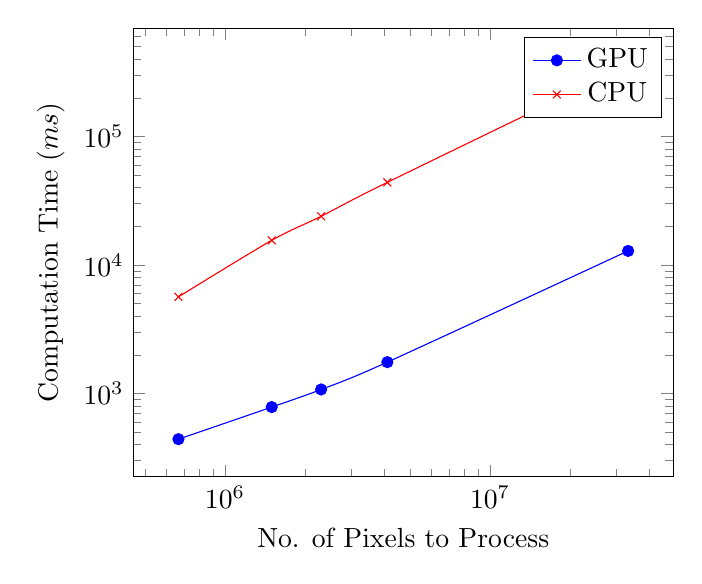
\begin{tikzpicture}
\begin{axis}[
    xlabel=$\text{\lr{No. of Pixels to Process}}$,
    ylabel=$\text{\lr{Computation Time }}(ms)$,
    xmin=0,
    ymin=0,
    xmode=log,
    ymode=log
%    xtick={10,20,30},
%    xticklabels={A,B,X},   % <---
%    ytick={0,10,...,100}
            ]
\addplot[smooth,mark=*,blue] plot coordinates {
    (667000,	441)
    (1500000,	784)
    (2304000,	1075)
    (4096000,	1754)
    (33177600,	12869)
};
\addlegendentry{\lr{GPU}}

\addplot[smooth,color=red,mark=x]
    plot coordinates {
        (667000,	5650)
        (1500000,	15557)
        (2304000,	23921)
        (4096000,	43963)
        (33177600,	356347)
    };
\addlegendentry{\lr{CPU}}
\end{axis}
\end{tikzpicture}
\caption{مقایسه‌ی زمان اجرای پیاده‌سازی‌های \lr{CPU} و \lr{GPU}.}
\label{Figure:Speed_Comparison}
\end{figure}

\end{document}